\label{sec:intro}

With the the development of hardwares and algorithms, the intellegence of a single agent has been greatly improved in recent years. 
The cooperation of agents can expand the capability of a unmanned system, and the multi-agent intelligent system is a promising reseach field.

Multi-robot exploration (MR-Explore), which provides the location and map for each robot, is the basic task of many multi-robot applications, such as multi-agent navigation and multi-agent rescue. 
For the keyword \textit{"robot"}, the feature-point extraction (FE) is a basic component for the visual odometry to estimate the 6 degree of freedom (6-DoF) pose.
For the keyword \textit{"multi"}, decentralized place recognition (PR), which translates an input image to a short representation code, is a fundamental element to produce candidate place matches.
Previous works use CNN to extract feature-points \cite{detone2018superpoint, simo2015discriminative, yi2016lift} and generate the representation code \cite{arandjelovic2016netvlad, radenovic2018fine}. The CNN-based feature-points from \cite{detone2018superpoint} reaches 10\%-30\% higher matching accuracy compared with the popular hand-crafted extraction method, ORB \cite{Mur-Artal:2017281}. The accuracy representation code from CNN-based method \cite{radenovic2018fine} is also ??\% better than the hand-crafted method [??].

\begin{figure}
	\centering
	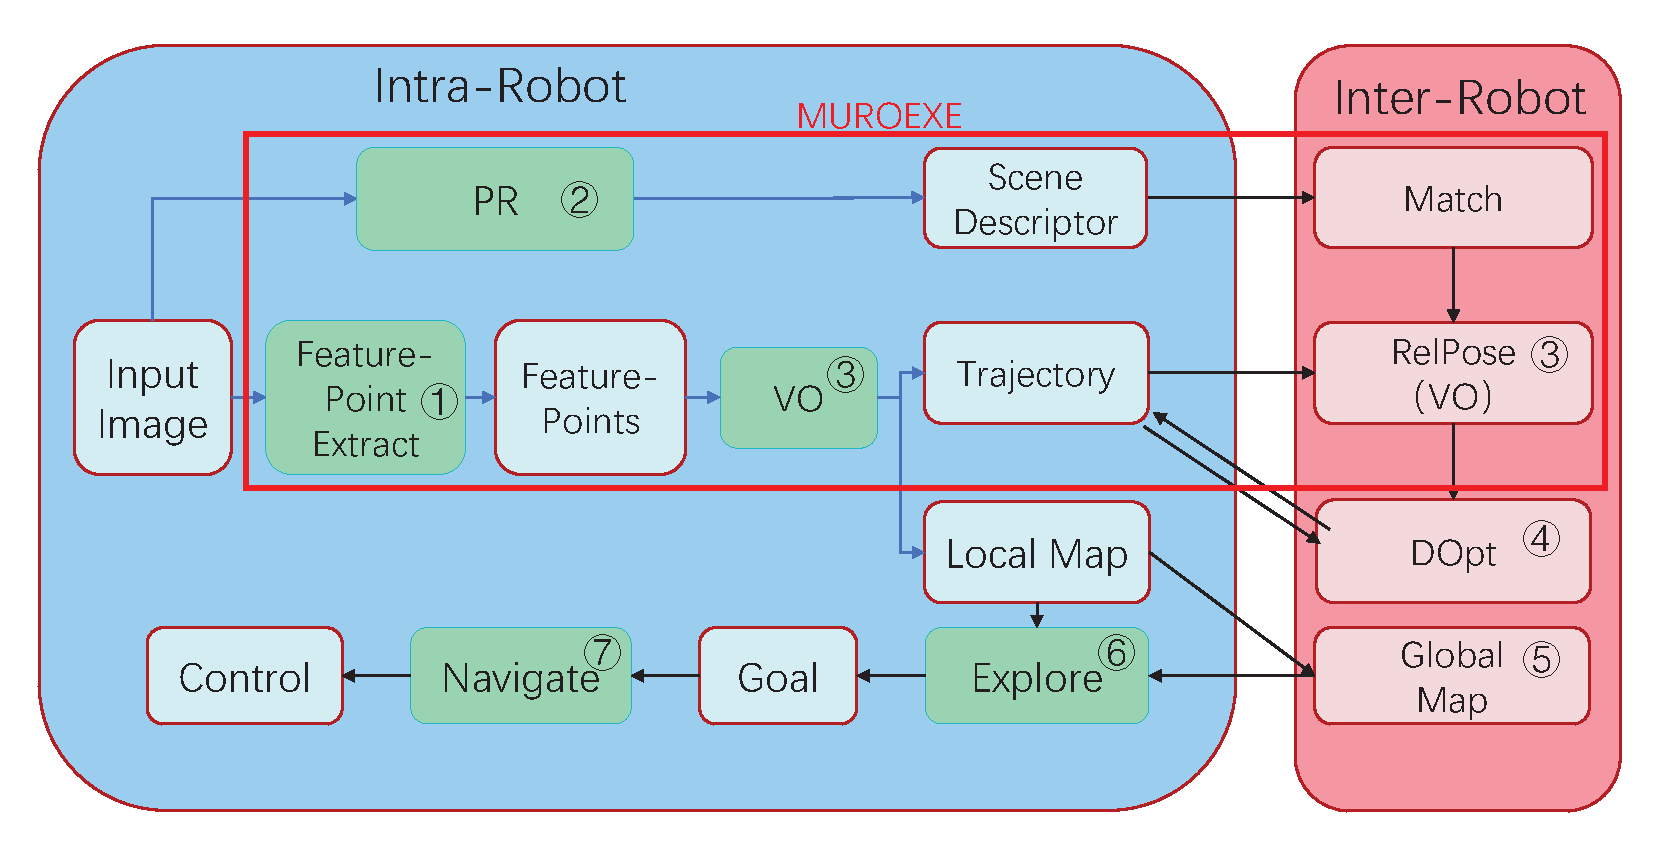
\includegraphics[width=0.99\linewidth]{fig/maexp.eps}
    \caption{
        The modules in MR-Explore. \textcircled{1}\textcircled{3} are basic for a single robot, should be execute every frame. \textcircled{2} generates representation code for some key frames. \textcircled{7}\textcircled{8} are only executed when representation codes are matched across robots and they are latency tolerant.  \textcircled{4}\textcircled{5}\textcircled{6} are for decision and navigation, also latency tolerant.
    }
	\label{fig:maexp}
\end{figure}

\Cref{fig:maexp} illustrates the computation modules in MR-Explore. Feature-point extraction (\textcircled{1}) and visual odometry (VO, \textcircled{3}) should be executed for each input frame, and should be finished before next frame.